\begin{frame}{integer representation}
    \begin{itemize}
        \item modern machine represent integers as series of \myemph{bits} (base-2)
        \item why not base-10?
    \end{itemize}
\end{frame}

\begin{frame}{ENIAC: base-10 representation}
\begin{tikzpicture}
\node (eniacPic) {
    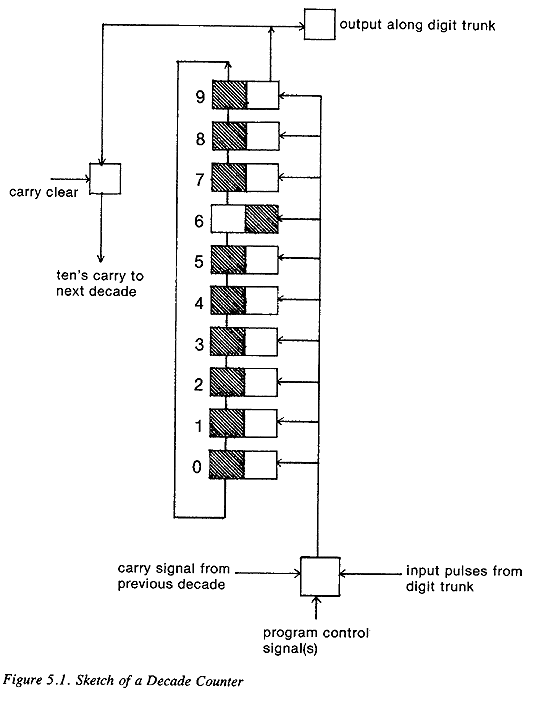
\includegraphics[width=7cm]{Reckoners-fig-05-01}
};
    \node[right=-2cm of eniacPic,align=left] {
        ENIAC: 1946 computer \\
        stored base-10 digits \\
        ~ \\
        ``ring counter'' of ten \\
        electronic switches per digit \\
   };
\begin{visibleenv}<2>
\draw[red,very thick,fill=red,fill opacity=0.05] ([xshift=2.5cm,yshift=-2.5cm]eniacPic.north west) rectangle ++(1.5cm,-1cm);
    \node[red,anchor=south west,inner sep=0mm,fill=white] at ([xshift=4.05cm,yshift=-2.7cm]eniacPic.north west) { flipped switch indicates digit stored };
\end{visibleenv}

\begin{visibleenv}<3>
    \node[red,anchor=south west,inner sep=0mm,fill=white,
        align=left] at ([xshift=4.05cm,yshift=-2cm]eniacPic.north west) {tens of vacuum tubes total \\(each $\sim$1¼\textquotedbl diameter by 2¾\textquotedbl height) };
\end{visibleenv}
\end{tikzpicture}
\end{frame}

% FIXME: base-2 switches

\begin{frame}{base-2 representation}
    \begin{itemize}
    \item base 2 --- each switch represents one ``digit''
        \begin{itemize}
        \item much more efficient use of switches
        \end{itemize}
    \item used in some pre-ENIAC electronic computers
        \begin{itemize}
        \item Atanasoff-Berry computer (1937, Ohio State)
        \item Z3 (1941, German Laboratory for Aviation)
        \end{itemize}
    \item<2-> why not used in ENIAC?
        \begin{itemize}
            \item \fontsize{8}{9}Eckert (ENIAC designer), 1953: ``Although [binary-based digit counters] were known at the time of the construction of the ENIAC, it was not used because it required stable resistors, which were then much more expensive than they are now.''
            \item also, important to input/output decimal digits directly
        \end{itemize}
    \end{itemize}
\imagecredit{quote: ``A Survey of Digital Computer Memory Systems'', Proceedings of the Institute of Radio Engineers, October 1953}
\end{frame}

\begin{frame}{base-2 bit addition}
\begin{tabular}{l|ll}
\textbf{+} & 0 & 1 \\
0 & 00 & \myemph<2>{01} \\
1 & \myemph<2>{01} & \myemph<2>{10} \\
\end{tabular}
\begin{itemize}
\item<2-> exactly one set to 1 --- result is 1; otherwise 0
\item<3-> both set to 1 --- carry is 1; otherwise 0
\end{itemize}
\end{frame}

\begin{frame}{base-2 capacity}
\begin{eqnarray*}
\text{$n$-bit number:}&\;&b_{n-1}b_{n-2}b_{n-3}\ldots b_2b_1b_0 \\
    & = & \sum_{i=0}^{n-1} b_i \cdot 2^i \\
    & \le & \sum_{i=0}^{n-1} 1 \cdot 2^i = \myemph<2>{2^{n-1}} \\
\end{eqnarray*}
\begin{itemize}
\item<3-> missing pieces:
    \begin{itemize}
    \item negative numbers?
    \item non-whole numbers?
    \item \myemph<4>{what is $n$?}
    \end{itemize}
\end{itemize}
\end{frame}

\begin{frame}{integer size in C++}
\begin{itemize}
\item varies between machines
    \begin{itemize}
    \item compiler uses what makes most sense on each machine?
    \end{itemize}
\end{itemize}
\begin{tabular}{l|l|l}
~ & \multicolumn{2}{c}{size in bits} \\
type & \myemph<3>{minimum} & on lab machines \\
\texttt{\myemph<2>{unsigned} char} & \myemph<3>{8} &  8 \\
\texttt{\myemph<2>{unsigned} short} & \myemph<3>{16} &  16 \\
\texttt{\myemph<2>{unsigned} int} & \myemph<3>{16} & 32 \\
\texttt{\myemph<2>{unsigned} long} & \myemph<3>{32} & 64 \\
\end{tabular}
\begin{tikzpicture}[overlay,remember picture]
\coordinate (place) at ([yshift=-3cm]current page.center);
\tikzset{
    box/.style={draw=red,fill=white,ultra thick,align=left,at=(place)},
}
\begin{visibleenv}<2>
\node[box] { ``unsigned'' --- can't be negative (no sign) };
\end{visibleenv}
\begin{visibleenv}<3>
\node[box] { minimum size required by standard for all C++ compilers \\
             all allowed to be bigger };
\end{visibleenv}
\end{tikzpicture}
\end{frame}

\begin{frame}[fragile,label=querySize]{querying sizes in C++}
\lstset{language=C++,style=smaller}
\begin{lstlisting}
#include <climits>  // C: <limits.h>
...
ULONG_MAX or UINT_MAX or USHRT_MAX or UCHAR_MAX
// e.g. USHRT_MAX == 65535 on lab machines
\end{lstlisting}
\hrule
\vspace{.5cm}
\begin{lstlisting}
#include <limits>  
...
std::numeric_limits<unsigned long>::max()
    // == ULONG_MAX
...
\end{lstlisting}
\vspace{.5cm}
\hrule
\begin{lstlisting}
sizeof(unsigned long)  // number of *bytes* 
    // == 8 on lab machines
...
\end{lstlisting}
\end{frame}
